% Options for packages loaded elsewhere
\PassOptionsToPackage{unicode}{hyperref}
\PassOptionsToPackage{hyphens}{url}
%
\documentclass[
  ignorenonframetext,
]{beamer}
\usepackage{pgfpages}
\setbeamertemplate{caption}[numbered]
\setbeamertemplate{caption label separator}{: }
\setbeamercolor{caption name}{fg=normal text.fg}
\beamertemplatenavigationsymbolsempty
% Prevent slide breaks in the middle of a paragraph
\widowpenalties 1 10000
\raggedbottom
\setbeamertemplate{part page}{
  \centering
  \begin{beamercolorbox}[sep=16pt,center]{part title}
    \usebeamerfont{part title}\insertpart\par
  \end{beamercolorbox}
}
\setbeamertemplate{section page}{
  \centering
  \begin{beamercolorbox}[sep=12pt,center]{part title}
    \usebeamerfont{section title}\insertsection\par
  \end{beamercolorbox}
}
\setbeamertemplate{subsection page}{
  \centering
  \begin{beamercolorbox}[sep=8pt,center]{part title}
    \usebeamerfont{subsection title}\insertsubsection\par
  \end{beamercolorbox}
}
\AtBeginPart{
  \frame{\partpage}
}
\AtBeginSection{
  \ifbibliography
  \else
    \frame{\sectionpage}
  \fi
}
\AtBeginSubsection{
  \frame{\subsectionpage}
}
\usepackage{amsmath,amssymb}
\usepackage{lmodern}
\usepackage{ifxetex,ifluatex}
\ifnum 0\ifxetex 1\fi\ifluatex 1\fi=0 % if pdftex
  \usepackage[T1]{fontenc}
  \usepackage[utf8]{inputenc}
  \usepackage{textcomp} % provide euro and other symbols
\else % if luatex or xetex
  \usepackage{unicode-math}
  \defaultfontfeatures{Scale=MatchLowercase}
  \defaultfontfeatures[\rmfamily]{Ligatures=TeX,Scale=1}
  \setmainfont[BoldFont = SF Pro Rounded Semibold]{SF Pro Rounded}
  \setmathfont[]{STIX Two Math}
\fi
\usefonttheme{serif} % use mainfont rather than sansfont for slide text
% Use upquote if available, for straight quotes in verbatim environments
\IfFileExists{upquote.sty}{\usepackage{upquote}}{}
\IfFileExists{microtype.sty}{% use microtype if available
  \usepackage[]{microtype}
  \UseMicrotypeSet[protrusion]{basicmath} % disable protrusion for tt fonts
}{}
\makeatletter
\@ifundefined{KOMAClassName}{% if non-KOMA class
  \IfFileExists{parskip.sty}{%
    \usepackage{parskip}
  }{% else
    \setlength{\parindent}{0pt}
    \setlength{\parskip}{6pt plus 2pt minus 1pt}}
}{% if KOMA class
  \KOMAoptions{parskip=half}}
\makeatother
\usepackage{xcolor}
\IfFileExists{xurl.sty}{\usepackage{xurl}}{} % add URL line breaks if available
\IfFileExists{bookmark.sty}{\usepackage{bookmark}}{\usepackage{hyperref}}
\hypersetup{
  pdftitle={444 Lecture 6.1 - Introducing Probability},
  pdfauthor={Brian Weatherson},
  hidelinks,
  pdfcreator={LaTeX via pandoc}}
\urlstyle{same} % disable monospaced font for URLs
\newif\ifbibliography
\usepackage{longtable,booktabs,array}
\usepackage{calc} % for calculating minipage widths
\usepackage{caption}
% Make caption package work with longtable
\makeatletter
\def\fnum@table{\tablename~\thetable}
\makeatother
\usepackage{graphicx}
\makeatletter
\def\maxwidth{\ifdim\Gin@nat@width>\linewidth\linewidth\else\Gin@nat@width\fi}
\def\maxheight{\ifdim\Gin@nat@height>\textheight\textheight\else\Gin@nat@height\fi}
\makeatother
% Scale images if necessary, so that they will not overflow the page
% margins by default, and it is still possible to overwrite the defaults
% using explicit options in \includegraphics[width, height, ...]{}
\setkeys{Gin}{width=\maxwidth,height=\maxheight,keepaspectratio}
% Set default figure placement to htbp
\makeatletter
\def\fps@figure{htbp}
\makeatother
\setlength{\emergencystretch}{3em} % prevent overfull lines
\providecommand{\tightlist}{%
  \setlength{\itemsep}{0pt}\setlength{\parskip}{0pt}}
\setcounter{secnumdepth}{-\maxdimen} % remove section numbering
\let\Tiny=\tiny

 \setbeamertemplate{navigation symbols}{} 

% \usetheme{Madrid}
 \usetheme[numbering=none, progressbar=foot]{metropolis}
 \usecolortheme{wolverine}
 \usepackage{color}
 \usepackage{MnSymbol}
% \usepackage{movie15}

\usepackage{amssymb}% http://ctan.org/pkg/amssymb
\usepackage{pifont}% http://ctan.org/pkg/pifont
\newcommand{\cmark}{\ding{51}}%
\newcommand{\xmark}{\ding{55}}%

\DeclareSymbolFont{symbolsC}{U}{txsyc}{m}{n}
\DeclareMathSymbol{\boxright}{\mathrel}{symbolsC}{128}
\DeclareMathAlphabet{\mathpzc}{OT1}{pzc}{m}{it}

\setlength{\parskip}{1ex plus 0.5ex minus 0.2ex}

\AtBeginSection[]
{
\begin{frame}
	\Huge{\color{darkblue} \insertsection}
\end{frame}
}

\renewenvironment*{quote}	
	{\list{}{\rightmargin   \leftmargin} \item } 	
	{\endlist }

\definecolor{darkgreen}{rgb}{0,0.7,0}
\definecolor{darkblue}{rgb}{0,0,0.8}

\usepackage[italic]{mathastext}
\usepackage{nicefrac}

\setbeamertemplate{caption}{\raggedright\insertcaption}

%\def\toprule{}
%\def\bottomrule{}
%\def\midrule{}
\usepackage{etoolbox}
\AfterEndEnvironment{description}{\vspace{9pt}}
\AfterEndEnvironment{oltableau}{\vspace{9pt}}
\BeforeBeginEnvironment{oltableau}{\vspace{9pt}}
\AfterEndEnvironment{center}{\vspace{9pt}}
\BeforeBeginEnvironment{tabular}{\vspace{9pt}}
\AfterEndEnvironment{longtable}{\vspace{-6pt}}
\usepackage{booktabs}
\usepackage{longtable}
\usepackage{array}
\usepackage{multirow}
\usepackage{wrapfig}
\usepackage{float}
\usepackage{colortbl}
\usepackage{pdflscape}
\usepackage{tabu}
\usepackage{threeparttable} 
\usepackage{threeparttablex} 
\usepackage[normalem]{ulem} 
\usepackage{makecell}
\usepackage{xcolor}
\usepackage{ulem}

\setlength\heavyrulewidth{0ex}
\setlength\lightrulewidth{0.08ex}

\aboverulesep=0ex
\belowrulesep=0ex
\renewcommand{\arraystretch}{1.2}
\ifluatex
  \usepackage{selnolig}  % disable illegal ligatures
\fi

\title{444 Lecture 6.1 - Introducing Probability}
\author{Brian Weatherson}
\date{}

\begin{document}
\frame{\titlepage}

\begin{frame}{Week Plan}
\protect\hypertarget{week-plan}{}
Pure revision/introduction of basics of probability
\end{frame}

\begin{frame}{Totally Not Compulsory}
\protect\hypertarget{totally-not-compulsory}{}
\begin{itemize}
\tightlist
\item
  If you've taken any college class using probability before, then
  probably 100\% of what I say this whole week will be pure revision.
\item
  I bet many people in the class could \emph{teach} all this stuff.
\item
  That's fine - take a week off.
\item
  But I really don't want anyone left behind before we dive into the
  more applied stuff.
\end{itemize}
\end{frame}

\begin{frame}{Book}
\protect\hypertarget{book}{}
\begin{figure}
\centering
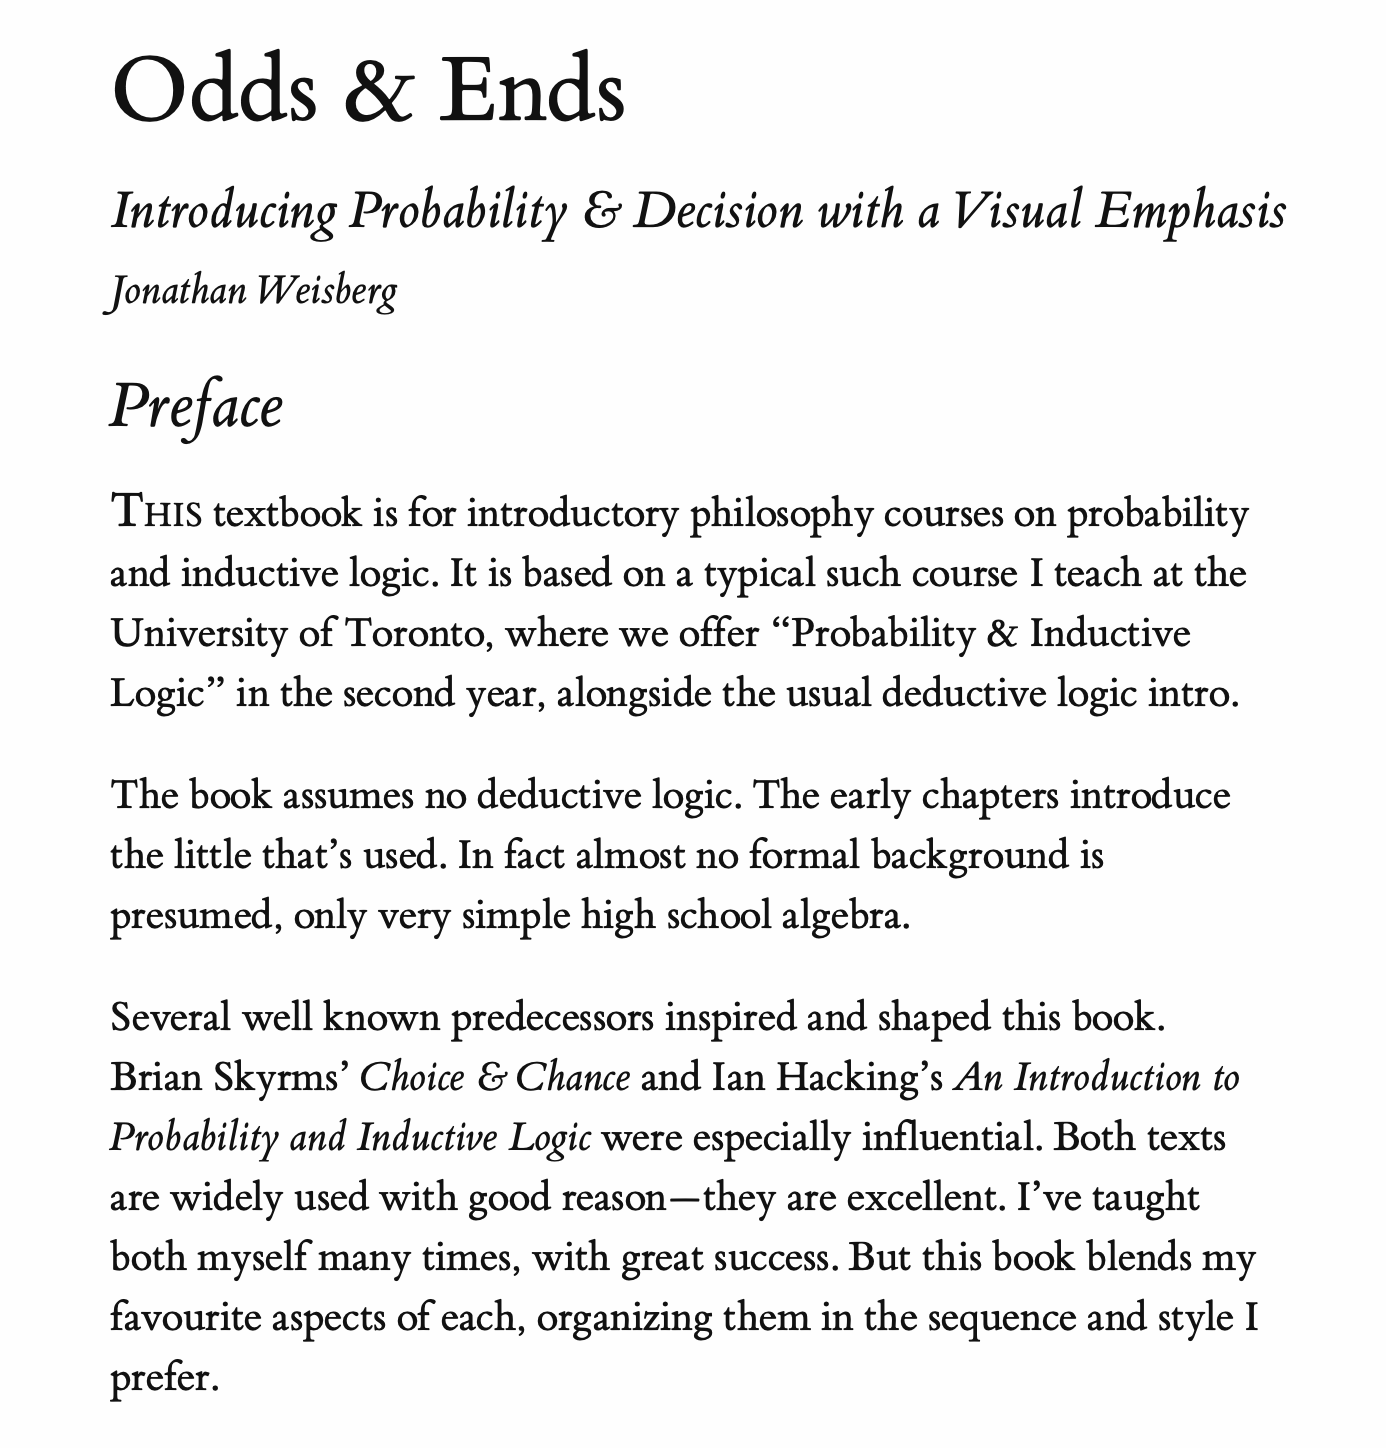
\includegraphics[width=\textwidth,height=0.7\textheight]{1_1_Odds_and_Ends.png}
\caption{These slides are based off an open access textbook, Odds and
Ends, available at \url{https://jonathanweisberg.org/vip/}}
\end{figure}
\end{frame}

\begin{frame}{Plan}
\protect\hypertarget{plan}{}
\begin{itemize}
\tightlist
\item
  This lecture introduces the basics of probability.
\end{itemize}
\end{frame}

\begin{frame}{Associated Reading}
\protect\hypertarget{associated-reading}{}
Odds and Ends, Chapter 1
\end{frame}

\begin{frame}{Basic Idea}
\protect\hypertarget{basic-idea}{}
\begin{itemize}
\tightlist
\item
  A probability function is a mapping from possibilities to numbers.
\item
  The numbers must sum to one.
\item
  Intuitively, the numbers measure how likely the possibilities are.
\end{itemize}
\end{frame}

\begin{frame}{Sum to One}
\protect\hypertarget{sum-to-one}{}
The math of probability functions is just the math of proportions.
Ultimately, all we'll be doing is the same kind of math that you would
do when thinking about things like

\begin{itemize}
\tightlist
\item
  What proportion of UM students are from North Carolina?
\item
  What proportion of UM undergraduates are Tigers fans?
\end{itemize}

etc.
\end{frame}

\begin{frame}{Three Big Questions}
\protect\hypertarget{three-big-questions}{}
\begin{enumerate}[<+->]
\tightlist
\item
  What to do with these numbers?
\item
  Where these numbers come from?
\item
  What do the numbers even mean?
\end{enumerate}
\end{frame}

\begin{frame}{A Simple Case}
\protect\hypertarget{a-simple-case}{}
\begin{itemize}
\tightlist
\item
  Imagine that it is basketball season, and UM has planned to have both
  the women's and men's teams play on the same night.
\item
  So at the end of the night there are four possible outcomes.
\end{itemize}
\end{frame}

\begin{frame}{Made Up Probabilities}
\protect\hypertarget{made-up-probabilities}{}
I'll stipulate that the probabilities of the four possible outcomes are
given by this table.

\begin{longtable}[]{@{}lcc@{}}
\toprule
& Men Win & Men Lose \\
\midrule
\endhead
Women Win & 0.45 & 0.25 \\
Women Lose & 0.20 & 0.10 \\
\bottomrule
\end{longtable}
\end{frame}

\begin{frame}{Another Representation}
\protect\hypertarget{another-representation}{}
Here are the same numbers written a different way.

\begin{longtable}[]{@{}ccc@{}}
\toprule
Women & Men & Probability \\
\midrule
\endhead
Win & Win & 0.45 \\
Win & Lose & 0.25 \\
Lose & Win & 0.20 \\
Lose & Lose & 0.10 \\
\bottomrule
\end{longtable}
\end{frame}

\begin{frame}{Possibilities}
\protect\hypertarget{possibilities}{}
Say a possibility (for current purposes) is one of these maximally
specific things that the probability is defined over.

\begin{itemize}
\tightlist
\item
  It is not really a complete possibility.
\item
  It doesn't tell us the score, or the weather, or the results of the
  next election, or for that matter the results of the last election.
\item
  But it tells us everything that's relevant to a particular inquiry.
\item
  It is a lot like a line on a truth table.
\end{itemize}
\end{frame}

\begin{frame}{Events}
\protect\hypertarget{events}{}
We will say an \textbf{event} is a proposition that can be defined using
these possibilities. So here are some sample events.

\begin{itemize}
\tightlist
\item
  The women's team wins.
\item
  The men's team wins.
\item
  At least one Michigan team wins.
\item
  The two teams have the same result.
\end{itemize}
\end{frame}

\begin{frame}{Probability of Events}
\protect\hypertarget{probability-of-events}{}
\begin{itemize}
\tightlist
\item
  An event is true at some possibilities, false at others.
\item
  Each possibility gets a probability.
\item
  The probability of an event is the sum of the probabilities of the
  possibilities where it is true.
\end{itemize}
\end{frame}

\begin{frame}{Examples - Probability Women's Team Wins}
\protect\hypertarget{examples---probability-womens-team-wins}{}
\begin{columns}[T]
\begin{column}{0.48\textwidth}
\begin{longtable}[]{@{}ccc@{}}
\toprule
Women & Men & Probability \\
\midrule
\endhead
Win & Win & 0.45 \\
Win & Lose & 0.25 \\
Lose & Win & 0.20 \\
Lose & Lose & 0.10 \\
\bottomrule
\end{longtable}
\end{column}

\begin{column}{0.48\textwidth}
\bigskip

\begin{itemize}
\tightlist
\item
  The women's team wins at lines 1 and 2.
\item
  So its probability is
\item
  0.45 + 0.25 = 0.7.
\end{itemize}
\end{column}
\end{columns}
\end{frame}

\begin{frame}{Examples - Probability Men's Team Wins}
\protect\hypertarget{examples---probability-mens-team-wins}{}
\begin{columns}[T]
\begin{column}{0.48\textwidth}
\begin{longtable}[]{@{}ccc@{}}
\toprule
Women & Men & Probability \\
\midrule
\endhead
Win & Win & 0.45 \\
Win & Lose & 0.25 \\
Lose & Win & 0.20 \\
Lose & Lose & 0.10 \\
\bottomrule
\end{longtable}
\end{column}

\begin{column}{0.48\textwidth}
\bigskip

\begin{itemize}
\tightlist
\item
  The men's team wins at lines 1 and 3.
\item
  So its probability is
\item
  0.45 + 0.20 = 0.65.
\end{itemize}
\end{column}
\end{columns}
\end{frame}

\begin{frame}{Examples - At Least One Team Wins}
\protect\hypertarget{examples---at-least-one-team-wins}{}
\begin{columns}[T]
\begin{column}{0.48\textwidth}
\begin{longtable}[]{@{}ccc@{}}
\toprule
Women & Men & Probability \\
\midrule
\endhead
Win & Win & 0.45 \\
Win & Lose & 0.25 \\
Lose & Win & 0.20 \\
Lose & Lose & 0.10 \\
\bottomrule
\end{longtable}
\end{column}

\begin{column}{0.48\textwidth}
\bigskip

\begin{itemize}
\tightlist
\item
  At least one team wins at lines 1, 2 and 3.
\item
  So its probability is
\item
  0.45 + 0.25 + 0.20 = 0.90.
\end{itemize}
\end{column}
\end{columns}
\end{frame}

\begin{frame}{Examples - Same Result in Each Game}
\protect\hypertarget{examples---same-result-in-each-game}{}
\begin{columns}[T]
\begin{column}{0.48\textwidth}
\begin{longtable}[]{@{}ccc@{}}
\toprule
Women & Men & Probability \\
\midrule
\endhead
Win & Win & 0.45 \\
Win & Lose & 0.25 \\
Lose & Win & 0.20 \\
Lose & Lose & 0.10 \\
\bottomrule
\end{longtable}
\end{column}

\begin{column}{0.48\textwidth}
\bigskip

\begin{itemize}
\tightlist
\item
  It is the same result in each game at lines 1 and 4.
\item
  So its probability is
\item
  0.45 + 0.10 = 0.55.
\end{itemize}
\end{column}
\end{columns}
\end{frame}

\begin{frame}{For Next Time}
\protect\hypertarget{for-next-time}{}
\begin{itemize}
\tightlist
\item
  We will look at some properties that all probability functions share.
\end{itemize}
\end{frame}

\end{document}
